\chapter{Misura della velocità della luce}

L'obiettivo del nostro esperimento è misurare la velocità della luce $c$.

L'apparato di misurazione consiste principalmente in:
\begin{itemize}
 \item Un laser Elio-Neon ($\lambda=32$ nm).
 \item Uno specchio rotante a velocità angolare regolabile.
 \item Due lenti convergenti, di lunghezza focale $l_1 = 48mm$ e $l_2 = 252 mm$.
 \item Un microscopio con beam splitter e micrometro.
\end{itemize}

Lo specchio rotante viene fatto girare con velocità angolare $\omega_1$ in senso orario e $\omega_2$ in senso antiorario. Queste velocità angolari sono identiche nella maggior parte dei casi, e la loro differenza è trascurabile.

Chiamando $s_{cw}$ e $s_{ccw}$ rispettivamente le misure con specchio rotante in senso orario e antiorario, per come è orientata la strumentazione il numero
$$\Delta s = s_{cw} - s_{ccw}$$
deve essere positivo.

Purtroppo però non è questo il caso per qualche misura presa in mattinata, per ragioni sconosciute e che non siamo riusciti a riprodurre. Questi dati sono esclusi dalla misurazione in quanto evidenti errori, e sono mostrati in rosso nel grafico seguente
I dati sono molti, dunque forniamo qui soltanto una visione grafica, e lasciamo la tabella come allegato.

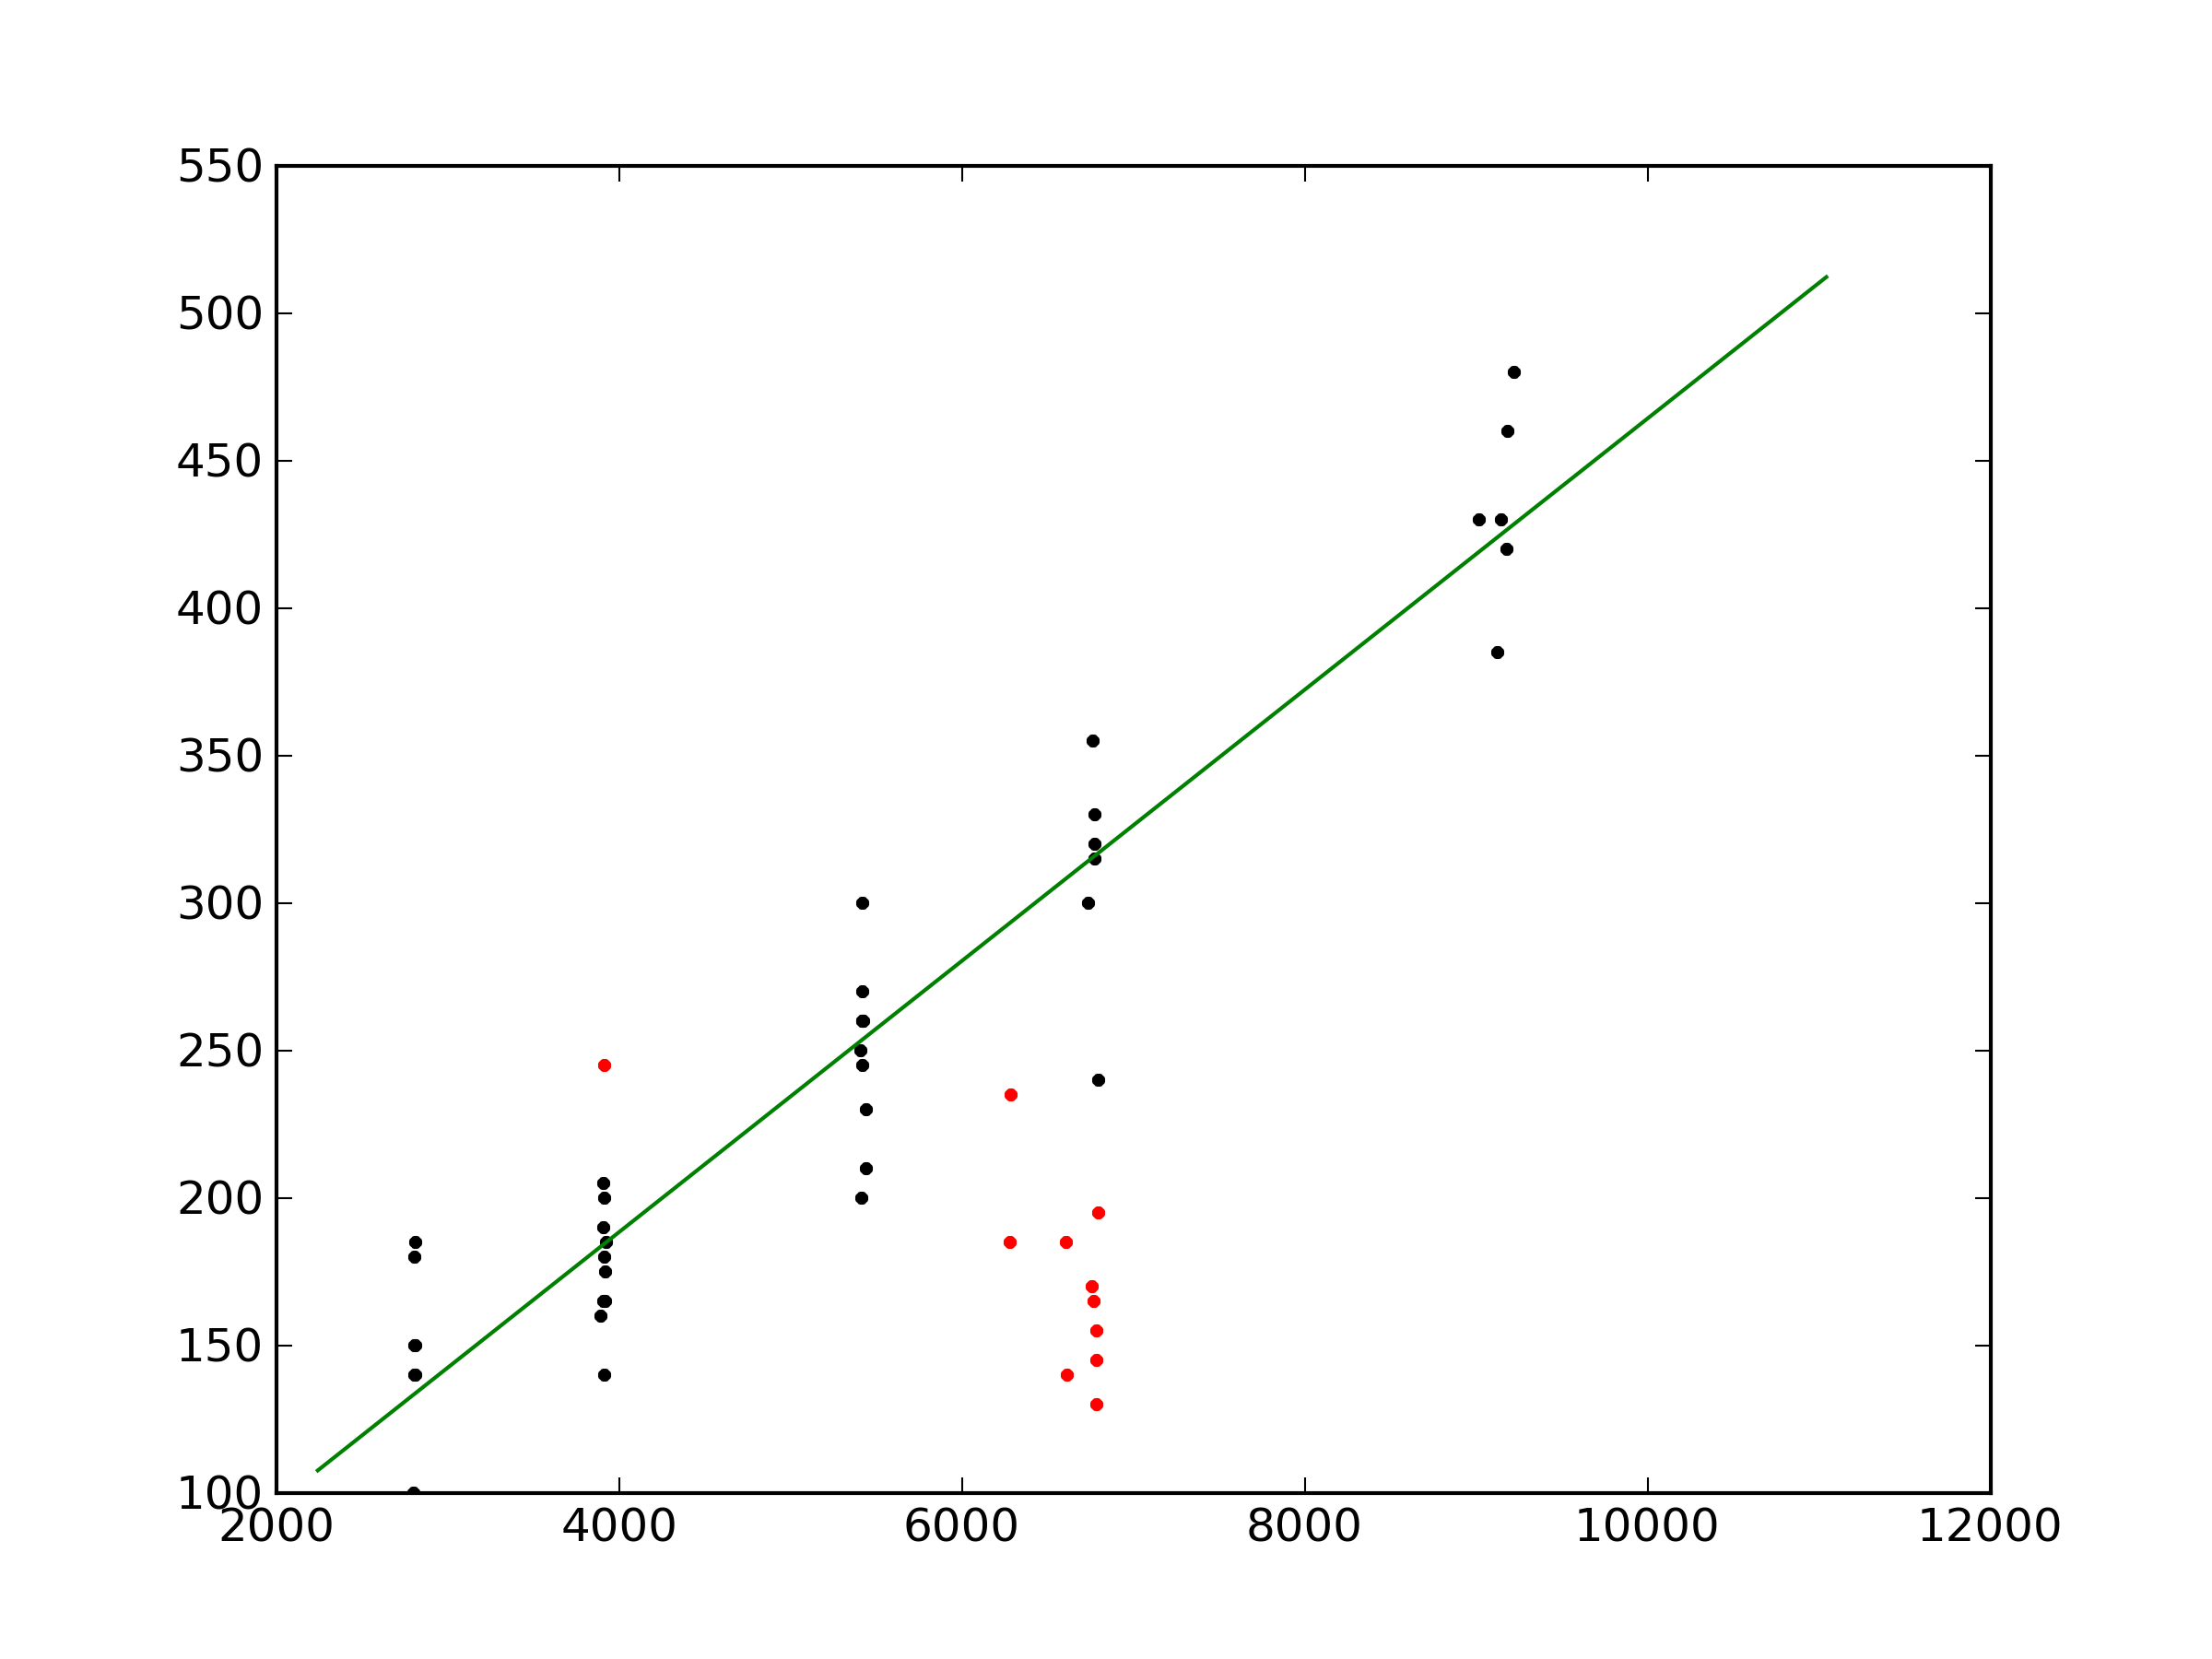
\includegraphics[scale=0.75]{grafici/C/dati.png}

\section{Analisi dati}

Data una 
m=0.04594423946498933

Ricaviamo, tramite  il fit della funzione $V=R*I$" dove R è parametro da stimare, due resistenze ignote.


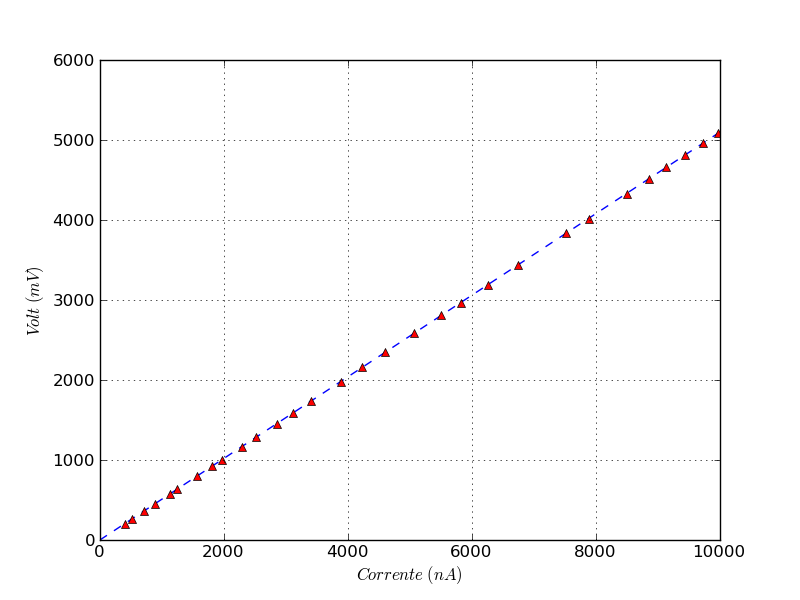
\includegraphics[scale=0.75]{grafici/C1/res1.png}
\

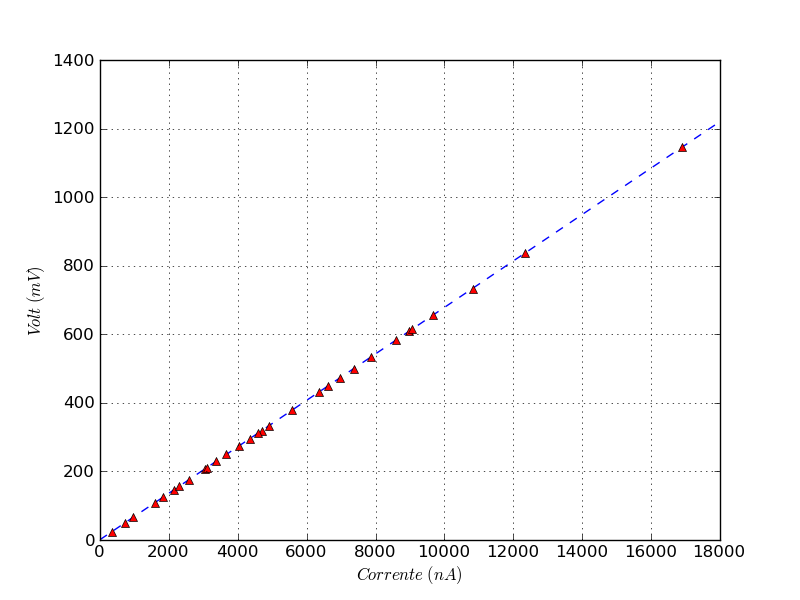
\includegraphics[scale=0.75]{grafici/C1/res2.png}

Misuro la resistenza interna del voltometro, mantenendo costante la ddp a $14.5\ V$ e variando la resistenza all'interno del circuito. 
Il voltmetro è in parallelo al circuito, perciò $R_i$:

$$R_i = \frac{RV}{RI-V} $$

dove R è la resistenza variabile, I la corrente nel circuito e $V= 14.5\ V$

\begin{center}
\begin{tabular}{*{2}{c}}
\end{tabular}

La resistenza risulta $9.20 \pm 0.27 \ M \Omega$.


Misuriamo la resistenza interna dell'amperometro, che è collegato in serie al circuito. 

$$R_i = \frac{V-RI}{I}$$

In questo caso, R è fissato ($R=0.5 \Omega$) e sono V e I a variare

La resistenza interna risulta $11.42 \pm 0.45 \Omega$


\end{center}


Colleghiamo una piccola lampada a filamento al circuito, e verifichiamo che il suo comportamento resistivo non segue la legge di Ohm. 





